%=================================================================
% CSE 4345 — Big Data Analytics
% Week 11, Part 1: Next Steps — Emerging Trends, Big Data Ethics,
%                  and Course Synthesis
% Department of CSE, Premier University
%
% Part 1 covers: Lakehouse architecture (Delta Lake, Iceberg) · Data
%               Mesh (Dehghani 2019) · MLOps pipelines · Edge analytics
%               · Cloud-native big data · Privacy-preserving analytics
%               · Course CLO synthesis map · Career pathways
%               · Apache Beam / Google Dataflow case study
%               · Ivy League alignment · Assessment pool
% Part 2 covers: Armbrust 2020 Delta Lake · Zaharia 2021 Lakehouse ·
%               Akidau 2015 Dataflow · Databricks vs Snowflake case study
%=================================================================

\documentclass[aspectratio=169,10pt]{beamer}

%---------- Packages ----------
\usepackage[utf8]{inputenc}
\usepackage[T1]{fontenc}
\usepackage{booktabs}
\usepackage{xcolor}
\usepackage{tikz}
\usetikzlibrary{shapes.geometric, positioning, arrows.meta,
                decorations.pathreplacing, calc, fit, backgrounds}
\usepackage{amsmath}
\usepackage{graphicx}
\usepackage{multicol}
\usepackage{enumerate}
\usepackage{array}
\usepackage{listings}

%---------- Theme ----------
\usetheme{Madrid}

%---------- Premier University Color Identity ----------
\definecolor{PUNavy}{RGB}{10,36,99}
\definecolor{PUGold}{RGB}{197,151,37}
\definecolor{PULightBlue}{RGB}{210,228,255}
\definecolor{PUTeal}{RGB}{0,100,100}
\definecolor{PUGray}{RGB}{90,90,90}
\definecolor{PURed}{RGB}{160,30,30}
\definecolor{PUGreen}{RGB}{30,120,60}
\definecolor{PUOrange}{RGB}{200,100,20}
\definecolor{PUPurple}{RGB}{80,0,120}

\setbeamercolor{palette primary}{bg=PUNavy, fg=white}
\setbeamercolor{palette secondary}{bg=PUNavy!85, fg=white}
\setbeamercolor{palette tertiary}{bg=PUNavy!70, fg=white}
\setbeamercolor{palette quaternary}{bg=PUNavy, fg=white}
\setbeamercolor{structure}{fg=PUNavy}
\setbeamercolor{title}{bg=PUNavy, fg=PUGold}
\setbeamercolor{subtitle}{fg=white}
\setbeamercolor{frametitle}{bg=PUNavy, fg=PUGold}
\setbeamercolor{alerted text}{fg=PUGold!85!black}
\setbeamercolor{block title}{bg=PUNavy, fg=white}
\setbeamercolor{block body}{bg=PULightBlue!45}
\setbeamercolor{block title alerted}{bg=PUGold!80!black, fg=white}
\setbeamercolor{block body alerted}{bg=PUGold!12}
\setbeamercolor{block title example}{bg=PUTeal, fg=white}
\setbeamercolor{block body example}{bg=PUTeal!10}
\setbeamercolor{section in toc}{fg=PUNavy}
\setbeamercolor{itemize item}{fg=PUGold!80!black}
\setbeamercolor{itemize subitem}{fg=PUNavy!70}

\setbeamertemplate{navigation symbols}{}
\setbeamertemplate{itemize item}{\scriptsize\raise1.5pt\hbox{\textbullet}}
\setbeamertemplate{itemize subitem}{\scriptsize\raise1pt\hbox{--}}

%---------- Code listing style ----------
\lstset{
  basicstyle=\ttfamily\scriptsize,
  backgroundcolor=\color{PUNavy!8},
  frame=single, rulecolor=\color{PUNavy!30},
  breaklines=true, language={},
  keywordstyle=\color{PUNavy}\bfseries,
  commentstyle=\color{PUGray}\itshape,
  stringstyle=\color{PUGreen!70!black},
}

%---------- Section separator ----------
\AtBeginSection[]{
  \begin{frame}[plain]
    \vfill\centering
    \begin{beamercolorbox}[sep=12pt,center,shadow=true,rounded=true]{block title}
      \usebeamerfont{title}\insertsectionhead\par
    \end{beamercolorbox}
    \vfill
  \end{frame}
}

%---------- Title metadata ----------
\title[CSE 4345 \textbar{} Week 11, Part 1]{CSE 4345: Big Data Analytics}
\subtitle{Week 11, Part 1 \textemdash\ Next Steps: Emerging Trends,
  Ethics \& Course Synthesis}
\author[Dept.\ of CSE]{Department of Computer Science \& Engineering\\[4pt]
       \small Premier University, Chittagong}
\institute{}
\date{Semester 2026}

%=================================================================
\begin{document}
%=================================================================

\begin{frame}\titlepage\end{frame}

%----------------------------------------------------------------
\begin{frame}{Course \& Lecture Information}
  \begin{columns}[T]
    \column{0.47\textwidth}
      \begin{block}{Lecture Identity}
        \begin{tabular}{ll}
          \textbf{Course:}      & CSE 4345 \\
          \textbf{Week / Part:} & 11 of 11 \textbar\ Part 1 of 2 \\
          \textbf{CLO:}         & CLO4 \\
          \textbf{PLO:}         & PLO(f) \\
        \end{tabular}
      \end{block}
      \vspace{6pt}
      \begin{alertblock}{CLO4}
        \textit{``Utilise the knowledge gained to solve big data problems and build a project applying big data tools and frameworks to real-world datasets''}
      \end{alertblock}
      \vspace{6pt}
      \begin{block}{Course Progression}
        \small
        Weeks 1--10: Foundations → storage → compute → query → pipelines → visualisation → real applications\\[4pt]
        \textbf{Week 11: Course synthesis, emerging trends, career pathways}\\[4pt]
        Big data is not a destination --- it is an evolving frontier.  The tools we taught represent the current mainstream; the field is shifting rapidly.
      \end{block}

    \column{0.50\textwidth}
      \begin{exampleblock}{Part 1 Covers}
        \begin{itemize}
          \item The \textbf{technology evolution arc}: Hadoop on-premise $\to$ cloud-native $\to$ Lakehouse
          \item \textbf{Lakehouse architecture}: Delta Lake, Apache Iceberg, ACID on object stores; unified BI + ML
          \item \textbf{Data Mesh}: decentralised domain-oriented data ownership (Dehghani 2019)
          \item \textbf{MLOps}: operationalising ML at scale --- MLflow, Airflow, Kubeflow, feature stores
          \item \textbf{Edge analytics}: processing at the IoT source --- AWS Greengrass, Azure IoT Edge
          \item \textbf{Privacy-preserving analytics}: federated learning, differential privacy
          \item \textbf{Generative AI on big data}: Text-to-SQL, RAG over data lakes
          \item Course CLO synthesis map; career pathways
          \item \textbf{Case study}: Google Dataflow / Apache Beam (Akidau 2015)
          \item Ivy League alignment; full assessment pool
        \end{itemize}
      \end{exampleblock}
  \end{columns}
\end{frame}

\begin{frame}{Lecture Agenda}\tableofcontents\end{frame}

%================================================================
\section{The Technology Evolution Arc}
%================================================================

\tikzset{
  earabox/.style={rectangle, rounded corners=4pt, minimum width=3.0cm,
                  minimum height=1.8cm, draw=PUNavy!25, font=\small,
                  align=center},
  earaarr/.style={-{Stealth[length=5pt]}, very thick, draw=PUNavy!60},
  earalbl/.style={font=\scriptsize\itshape, text=PUGray}
}
\begin{frame}{How Big Data Technology Has Evolved: 2003 -- 2025}
  \begin{center}
  \begin{tikzpicture}
    % Era boxes (background rectangles)
    \node[earabox, fill=PUNavy!15] (e1) at (-5.2, 0) {};
    \node[earabox, fill=PUGold!20] (e2) at (-1.7, 0) {};
    \node[earabox, fill=PUGreen!20] (e3) at (1.8, 0) {};
    \node[earabox, fill=PURed!15, draw=PURed!40] (e4) at (5.3, 0) {};

    % Era 1 labels
    \node[font=\small\bfseries] at (-5.2, 0.65) {Era 1};
    \node[font=\scriptsize]     at (-5.2, 0.25) {2003--2011};
    \node[font=\scriptsize]     at (-5.2,-0.15) {GFS, MapReduce};
    \node[font=\scriptsize]     at (-5.2,-0.50) {Hadoop, Hive};
    \node[font=\scriptsize]     at (-5.2,-0.85) {On-premise};
    % Era 2 labels
    \node[font=\small\bfseries] at (-1.7, 0.65) {Era 2};
    \node[font=\scriptsize]     at (-1.7, 0.25) {2011--2017};
    \node[font=\scriptsize]     at (-1.7,-0.15) {Spark, Kafka};
    \node[font=\scriptsize]     at (-1.7,-0.50) {YARN, Parquet};
    \node[font=\scriptsize]     at (-1.7,-0.85) {Batch + stream};
    % Era 3 labels
    \node[font=\small\bfseries] at (1.8, 0.65) {Era 3};
    \node[font=\scriptsize]     at (1.8, 0.25) {2017--2022};
    \node[font=\scriptsize]     at (1.8,-0.15) {Cloud-native};
    \node[font=\scriptsize]     at (1.8,-0.50) {S3, EMR, Dataproc};
    \node[font=\scriptsize]     at (1.8,-0.85) {Managed services};
    % Era 4 labels
    \node[font=\small\bfseries] at (5.3, 0.65) {Era 4};
    \node[font=\scriptsize]     at (5.3, 0.25) {2022 -- now};
    \node[font=\scriptsize]     at (5.3,-0.15) {Lakehouse, Mesh};
    \node[font=\scriptsize]     at (5.3,-0.50) {MLOps, Edge, GenAI};
    \node[font=\scriptsize]     at (5.3,-0.85) {ACID on obj. stores};

    \draw[earaarr] (e1)--(e2);
    \draw[earaarr] (e2)--(e3);
    \draw[earaarr] (e3)--(e4);

    \node[earalbl] at (-3.45, -1.6) {Spark kills MR};
    \node[earalbl] at (0.05, -1.6) {cloud kills HDFS};
    \node[earalbl] at (3.55, -1.6) {LLMs reshape queries};

    % Key papers band
    \node[rectangle, fill=PUGray!10, draw=PUGray!30, rounded corners=3pt,
          minimum width=13.5cm, minimum height=0.5cm,
          font=\scriptsize] at (0, -2.5) {%
          GFS '03 · MR '04 · Hive '09 · Spark '10 · Kafka '11 · YARN '13 ·
          Dataflow '15 · Delta Lake '20 · Lakehouse '21};
  \end{tikzpicture}
  \end{center}
  \vspace{4pt}
  \begin{alertblock}{\small Key Insight for Practitioners}
    \small Tools from Era 1 (HDFS, MapReduce) are still running in production at large enterprises.  Technologies do not die when they are superseded --- they \textit{stratify} into legacy tiers.  Understanding the full arc is essential for a Big Data Architect who must maintain old systems while migrating to new ones.
  \end{alertblock}
\end{frame}

%================================================================
\section{Lakehouse Architecture}
%================================================================

\begin{frame}{Lakehouse: Unifying Data Lakes and Data Warehouses}
  \begin{columns}[T]
    \column{0.52\textwidth}
      \begin{block}{The Problem: Two Architectures, Two Pain Points}
        \small
        \textbf{Data Lake (pure):}  Raw files on S3 / HDFS.  Cheap storage, supports any format.
        But: \textbf{no ACID transactions} (concurrent writes corrupt data), \textbf{no schema enforcement} (data swamp risk), slow BI queries (no indexing).

        \vspace{6pt}
        \textbf{Data Warehouse (Hive / Redshift):}  ACID, schema-on-write, fast BI.
        But: proprietary format locks in vendor, ML teams cannot access raw data, expensive to store all historical data.

        \vspace{6pt}
        \textbf{Lakehouse} (Zaharia et al., CIDR 2021):
        \begin{itemize}
          \item Open table format (\textbf{Delta Lake}, Apache \textbf{Iceberg}, Apache \textbf{Hudi}) sits on top of cheap object storage (S3 / Azure ADLS)
          \item Provides \textbf{ACID transactions}, \textbf{time travel} (query data as of any past point), \textbf{schema evolution}, and \textbf{audit logging} --- all via a transaction log in the same object store
          \item BI tools (Tableau, Superset) and ML frameworks (Spark MLlib, PyTorch) query the \textbf{same data} via Spark SQL or DuckDB
        \end{itemize}
      \end{block}

    \column{0.45\textwidth}
      \begin{center}
      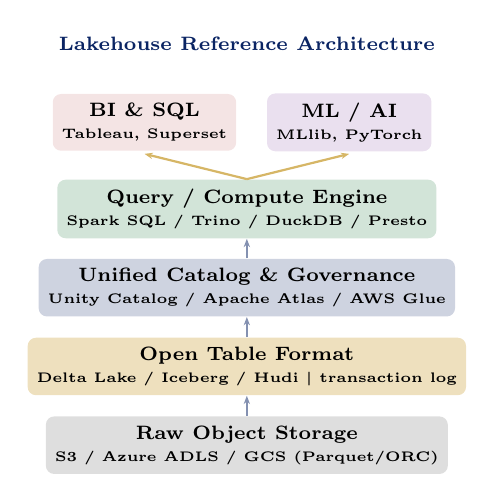
\begin{tikzpicture}[
          lyr/.style={rectangle, rounded corners=3pt, minimum width=4.2cm,
                      minimum height=0.7cm, font=\scriptsize\bfseries,
                      align=center},
          arr/.style={-{Stealth[length=3pt]}, thick, draw=PUNavy!50}
        ]
        \node[font=\scriptsize\bfseries, PUNavy] at (0, 5.5)
              {Lakehouse Reference Architecture};

        % Layers bottom to top
        \node[lyr, fill=PUGray!20]     (raw)  at (0, 0.4)
              {Raw Object Storage\\{\tiny S3 / Azure ADLS / GCS (Parquet/ORC)}};

        \node[lyr, fill=PUGold!30]     (tlog) at (0, 1.4)
              {Open Table Format\\{\tiny Delta Lake / Iceberg / Hudi \textbar\ transaction log}};

        \node[lyr, fill=PUNavy!20]     (cat)  at (0, 2.4)
              {Unified Catalog \& Governance\\{\tiny Unity Catalog / Apache Atlas / AWS Glue}};

        \node[lyr, fill=PUGreen!20]    (eng)  at (0, 3.4)
              {Query / Compute Engine\\{\tiny Spark SQL / Trino / DuckDB / Presto}};

        \draw[arr] (raw)--(tlog);
        \draw[arr] (tlog)--(cat);
        \draw[arr] (cat)--(eng);

        % Consumers
        \node[lyr, fill=PURed!12, minimum width=1.9cm]
              (bi) at (-1.3, 4.5) {BI \& SQL\\{\tiny Tableau, Superset}};
        \node[lyr, fill=PUPurple!12, minimum width=1.9cm]
              (ml) at (1.3, 4.5) {ML / AI\\{\tiny MLlib, PyTorch}};

        \draw[arr, PUGold!70] (eng.north) -- (-1.3, 4.1);
        \draw[arr, PUGold!70] (eng.north) -- (1.3, 4.1);
      \end{tikzpicture}
      \end{center}
  \end{columns}
\end{frame}

%----------------------------------------------------------------
\begin{frame}{Delta Lake and Apache Iceberg: ACID on Object Stores}
  \begin{columns}[T]
    \column{0.52\textwidth}
      \begin{block}{How Delta Lake Achieves ACID}
        Delta Lake (Armbrust et al., VLDB 2020) stores a \textbf{transaction log} (a set of JSON files called the \textbf{delta log}) alongside the Parquet data files in S3:
        \begin{enumerate}
          \item Every write appends a new \textbf{commit entry} to the delta log listing: files added, files deleted, schema changes, metadata
          \item Readers look up the latest committed state from the log before scanning data files --- \textbf{snapshot isolation}
          \item If two writers try to commit conflicting changes simultaneously, the second writer's optimistic concurrency check fails and it retries --- \textbf{serialisable writes}
          \item \textbf{Time travel:} Query data as of any previous snapshot: \texttt{VERSION AS OF 42} or \texttt{TIMESTAMP AS OF `2025-01-01`}
        \end{enumerate}
        \vspace{4pt}
        Apache \textbf{Iceberg} (Netflix) and Apache \textbf{Hudi} (Uber) solve the same problem with different trade-offs in partition evolution and upsert performance.
      \end{block}

    \column{0.45\textwidth}
      \begin{exampleblock}{Data Lakehouse vs Alternatives}
        {\small
        \renewcommand{\arraystretch}{1.35}
        \begin{tabular}{p{1.5cm}p{1.2cm}p{1.2cm}p{1.5cm}}
          \toprule
          & \textbf{Data Lake} & \textbf{DW} & \textbf{Lakehouse} \\
          \midrule
          ACID         & No     & Yes   & \textbf{Yes} \\
          Open format  & Yes    & No    & \textbf{Yes} \\
          BI queries   & Slow   & Fast  & \textbf{Fast} \\
          ML / raw     & Yes    & No    & \textbf{Yes} \\
          Storage cost & Low    & High  & \textbf{Low} \\
          Schema enf.  & No     & Yes   & \textbf{Yes} \\
          \bottomrule
        \end{tabular}
        }
        \vspace{6pt}
        \textbf{Bangladesh context:}  bKash's transaction data (50 M transactions/day, 5+ years of history) is a candidate Lakehouse workload: compliance audits need ACID and time travel; fraud ML models need raw Parquet; monthly BI dashboards need fast SQL --- three requirements that only a Lakehouse satisfies simultaneously.
      \end{exampleblock}
  \end{columns}
\end{frame}

%================================================================
\section{Data Mesh}
%================================================================

\begin{frame}[fragile]{Data Mesh: Decentralised Domain-Oriented Data Ownership}
  \begin{columns}[T]
    \column{0.52\textwidth}
      \begin{block}{Why Centralised Data Platforms Create Bottlenecks}
        In the traditional model, a \textbf{central data engineering team} ingests data from every business domain, builds pipelines, and publishes datasets.  At scale, this creates:
        \begin{itemize}
          \item \textbf{Ownership mismatch:} the team that built the pipeline does not understand the domain; the domain team that understands the data cannot change the pipeline
          \item \textbf{Queue bottleneck:} 200 teams competing for 20 data engineers
          \item \textbf{Quality degradation:} nobody is accountable for downstream data correctness
        \end{itemize}
        \vspace{4pt}
        \textbf{Data Mesh} (Zhamak Dehghani, 2019 / 2022) is a \textbf{sociotechnical paradigm} with four principles:
        \begin{enumerate}
          \item \textbf{Domain ownership:} each business domain owns, publishes, and is SLA-accountable for its own data product
          \item \textbf{Data as a product:} data is discoverable, addressable, trustworthy, and self-describing
          \item \textbf{Self-serve data platform:} infrastructure abstractions so domain teams need no Spark expertise
          \item \textbf{Federated computational governance:} global policies (GDPR, PDPA) enforced automatically, local flexibility preserved
        \end{enumerate}
      \end{block}

    \column{0.45\textwidth}
      \begin{center}
      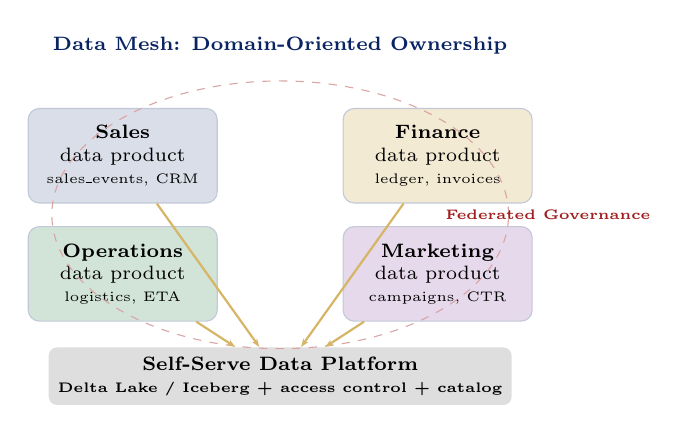
\begin{tikzpicture}[
          dom/.style={rectangle, rounded corners=4pt, minimum width=2.4cm,
                      minimum height=1.2cm, draw=PUNavy!25, font=\scriptsize,
                      align=center},
          pl/.style={rectangle, rounded corners=3pt, minimum width=5.4cm, minimum height=0.7cm, font=\scriptsize\bfseries, align=center},
          arr/.style={-{Stealth[length=3pt]}, draw=PUGold!70, thick}
        ]
        \node[font=\scriptsize\bfseries, PUNavy] at (0, 5.2)
              {Data Mesh: Domain-Oriented Ownership};

        \node[dom, fill=PUNavy!15]   (sales) at (-2.0, 3.8)
              {\textbf{Sales}\\data product\\{\tiny sales\_events, CRM}};
        \node[dom, fill=PUGold!20]   (fin)   at (2.0, 3.8)
              {\textbf{Finance}\\data product\\{\tiny ledger, invoices}};
        \node[dom, fill=PUGreen!20]  (ops)   at (-2.0, 2.3)
              {\textbf{Operations}\\data product\\{\tiny logistics, ETA}};
        \node[dom, fill=PUPurple!15] (mkt)   at (2.0, 2.3)
              {\textbf{Marketing}\\data product\\{\tiny campaigns, CTR}};

        % Self-serve platform
        \node[pl, fill=PUGray!20] (plat) at (0, 1.0)
              {Self-Serve Data Platform\\{\tiny Delta Lake / Iceberg + access control + catalog}};

        % Governance ring
        \node[ellipse, draw=PURed!40, dashed, minimum width=5.8cm,
              minimum height=3.4cm] at (0, 3.05) {};
        \node[font=\tiny\bfseries, PURed] at (3.4, 3.05)
              {Federated Governance};

        \foreach \d in {sales, fin, ops, mkt} {
          \draw[arr] (\d)--(plat);
        }
      \end{tikzpicture}
      \end{center}
  \end{columns}
\end{frame}

%================================================================
\section{MLOps and Feature Stores}
%================================================================

\begin{frame}{MLOps: From Experiment to Production ML}
  \begin{columns}[T]
    \column{0.52\textwidth}
      \begin{block}{The Hidden Debt in ML Systems (Sculley et al., NeurIPS 2015)}
        ``Only a small fraction of real-world ML systems is composed of the ML code.  The required surrounding infrastructure is vast and complex.''
        \vspace{4pt}
        A trained model that lives only in a Jupyter notebook delivers zero business value.  \textbf{MLOps} (ML Operations) is the discipline of reliably \textbf{deploying}, \textbf{monitoring}, and \textbf{retraining} models in production:
        \begin{itemize}
          \item \textbf{Data pipeline:} reproducible feature engineering (Apache Airflow DAGs)
          \item \textbf{Experiment tracking:} log hyperparameters, metrics, and artefacts (\textbf{MLflow})
          \item \textbf{Feature store:} centralised repository of reusable features shared across teams; prevents training--serving skew (\textbf{Feast}, \textbf{Tecton})
          \item \textbf{Model registry:} version-controlled catalogue of trained models with staging / production labels (\textbf{MLflow Model Registry})
          \item \textbf{Serving:} REST API endpoints with canary deployment (\textbf{KServe}, \textbf{Seldon})
          \item \textbf{Monitoring:} detect data drift and model performance decay (\textbf{Evidently}, \textbf{Arize})
        \end{itemize}
      \end{block}

    \column{0.45\textwidth}
      \begin{center}
      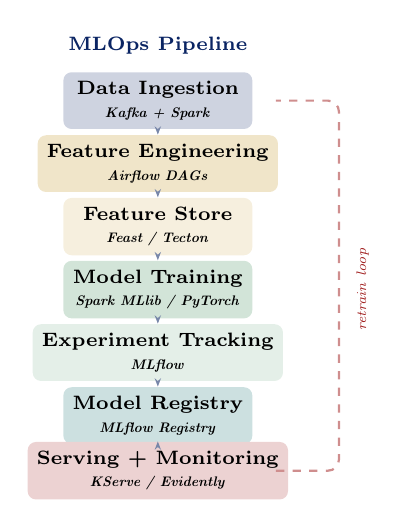
\begin{tikzpicture}[
          box/.style={rectangle, rounded corners=3pt, minimum width=2.4cm,
                      minimum height=0.65cm, font=\scriptsize\bfseries, align=center},
          arr/.style={-{Stealth[length=3pt]}, thick, draw=PUNavy!55}
        ]
        \node[font=\scriptsize\bfseries, PUNavy] at (0, 5.5)
              {MLOps Pipeline};

        \node[box, fill=PUNavy!20] (na) at (0, 4.8)
              {Data Ingestion\\\textit{\tiny Kafka + Spark}};
        \node[box, fill=PUGold!25] (nb) at (0, 4.0)
              {Feature Engineering\\\textit{\tiny Airflow DAGs}};
        \node[box, fill=PUGold!15] (nc) at (0, 3.2)
              {Feature Store\\\textit{\tiny Feast / Tecton}};
        \node[box, fill=PUGreen!20] (nd) at (0, 2.4)
              {Model Training\\\textit{\tiny Spark MLlib / PyTorch}};
        \node[box, fill=PUGreen!12] (ne) at (0, 1.6)
              {Experiment Tracking\\\textit{\tiny MLflow}};
        \node[box, fill=PUTeal!20] (nf) at (0, 0.8)
              {Model Registry\\\textit{\tiny MLflow Registry}};
        \node[box, fill=PURed!20] (ng) at (0, 0.1)
              {Serving + Monitoring\\\textit{\tiny KServe / Evidently}};

        \foreach \a/\b in {na/nb, nb/nc, nc/nd, nd/ne, ne/nf, nf/ng} {
          \draw[arr] (\a)--(\b);
        }

        % Feedback loop
        \draw[PURed!50, thick, dashed, rounded corners=4pt]
          (1.5, 0.1) -- (2.3, 0.1) -- (2.3, 4.8) -- (1.5, 4.8);
        \node[font=\tiny\itshape, PURed, rotate=90] at (2.6, 2.4)
              {retrain loop};
      \end{tikzpicture}
      \end{center}
  \end{columns}
\end{frame}

%================================================================
\section{Edge Analytics and Cloud-Native Big Data}
%================================================================

\begin{frame}{Edge Analytics: Pushing Computation to the Data Source}
  \begin{columns}[T]
    \column{0.52\textwidth}
      \begin{block}{Why Edge?}
        The IoT data generation model (wearables, industrial sensors, CCTV cameras, RMG factory floor monitors) creates a \textbf{bandwidth and latency bottleneck}: transmitting every raw sensor reading to a central cloud cluster is impractical.

        \vspace{4pt}
        \textbf{Edge analytics} places lightweight compute \textit{at or near} the source:
        \begin{itemize}
          \item \textbf{Tier 1 (device):} pre-processing, filtering, anomaly detection on microcontroller or FPGA (e.g., TensorFlow Lite on a wearable ECG patch)
          \item \textbf{Tier 2 (edge gateway):} local aggregation, windowed statistics, pre-trained model inference.  Only summary events are forwarded to the cloud.  \textit{Example:} AWS Greengrass on a factory-floor server; Azure IoT Edge on an RMG weaving machine controller
          \item \textbf{Tier 3 (cloud):} global model retraining on aggregated data from all edge nodes; long-term storage; BI dashboards
        \end{itemize}

        \vspace{4pt}
        \textbf{Bangladesh:} DESCO power grid substations generate 100{,}000 voltage readings/second.  Edge nodes run Isolation Forest locally, sending only anomaly alerts (3--5 events/minute) to the national grid monitoring centre.
      \end{block}

    \column{0.45\textwidth}
      \begin{center}
      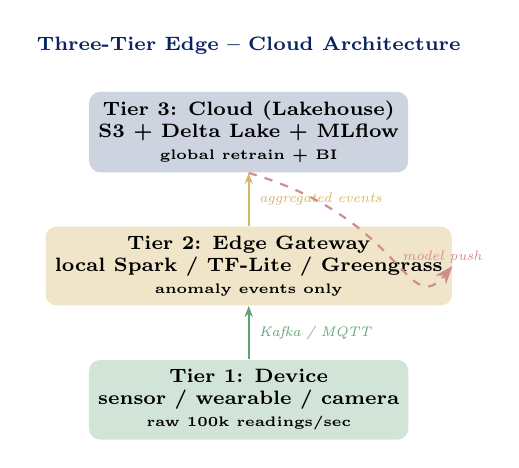
\begin{tikzpicture}[
          tier/.style={rectangle, rounded corners=4pt, minimum width=3.6cm,
                       minimum height=0.9cm, font=\scriptsize\bfseries, align=center},
          arr/.style={-{Stealth[length=4pt]}, thick}
        ]
        \node[font=\scriptsize\bfseries, PUNavy] at (0, 5.0)
              {Three-Tier Edge -- Cloud Architecture};

        % Tier 1
        \node[tier, fill=PUGreen!20] (t1) at (0, 0.5)
              {Tier 1: Device\\{\scriptsize sensor / wearable / camera}\\{\tiny raw 100k readings/sec}};
        % Tier 2
        \node[tier, fill=PUGold!25] (t2) at (0, 2.2)
              {Tier 2: Edge Gateway\\{\scriptsize local Spark / TF-Lite / Greengrass}\\{\tiny anomaly events only}};
        % Tier 3
        \node[tier, fill=PUNavy!20] (t3) at (0, 3.9)
              {Tier 3: Cloud (Lakehouse)\\{\scriptsize S3 + Delta Lake + MLflow}\\{\tiny global retrain + BI}};

        \draw[arr, PUGreen!70] (t1)--(t2)
              node[midway, right, font=\tiny\itshape]{Kafka / MQTT};
        \draw[arr, PUGold!70]  (t2)--(t3)
              node[midway, right, font=\tiny\itshape]{aggregated events};
        \draw[PURed!50, dashed, thick, -Stealth]
              (t3.south) .. controls (2.0,2.8) and (2.0,1.5) .. (t2.east)
              node[midway, right, font=\tiny\itshape]{model push};
      \end{tikzpicture}
      \end{center}
      \vspace{4pt}
      \begin{alertblock}{Cloud-Native Big Data}
        \small On-premise Hadoop clusters are being replaced by \textbf{managed cloud services}: AWS EMR, Google Dataproc, Azure HDInsight.  No hardware to provision; auto-scaling to zero when idle.  Separation of storage (S3) and compute (ephemeral EMR cluster) reduces cost by 60--80\% for batch workloads.
      \end{alertblock}
  \end{columns}
\end{frame}

%================================================================
\section{Privacy-Preserving Analytics}
%================================================================

\begin{frame}{Federated Learning and Differential Privacy}
  \begin{columns}[T]
    \column{0.52\textwidth}
      \begin{block}{Federated Learning: Train Without Sharing Data}
        In healthcare, finance, and government, \textbf{raw data cannot leave organisational boundaries} due to regulation (HIPAA, PDPA Bangladesh, GDPR).  \textbf{Federated Learning} (McMahan et al., Google 2017) enables:
        \begin{enumerate}
          \item A \textbf{global model} is pushed to each participating hospital / bank
          \item Each institution trains the model on its \textbf{local data} only
          \item Only \textbf{model weight updates} (gradients) --- not raw patient records --- are sent to a central aggregation server
          \item The server applies \textbf{FedAvg} (weighted average of gradients) to update the global model
          \item Repeat for multiple rounds until convergence
        \end{enumerate}
        \vspace{4pt}
        \textbf{Bangladesh application:}  DGHS + five major private hospital networks jointly train an ICU mortality prediction model via federated learning --- combining 200{,}000 patient records without any hospital ever sharing individual records with another.
      \end{block}

    \column{0.45\textwidth}
      \begin{exampleblock}{Differential Privacy: Provable Anonymisation}
        \small A mechanism $\mathcal{M}$ satisfies \textbf{$(\varepsilon, \delta)$-differential privacy} if removing or adding any single individual's record changes the output distribution by at most a factor of $e^\varepsilon$ (with probability $1-\delta$).
        \vspace{4pt}

        \textbf{In practice:}  Add \textbf{Laplace noise} (calibrated to sensitivity $\Delta f$ and privacy budget $\varepsilon$) to aggregate query results before publishing:
        \[
          \tilde{f}(D) = f(D) + \text{Lap}\!\left(\frac{\Delta f}{\varepsilon}\right)
        \]

        Smaller $\varepsilon$ $\Rightarrow$ more privacy, less accuracy.  The privacy budget is ``spent'' with each query.

        \vspace{4pt}
        \textbf{Real deployments:}
        \begin{itemize}
          \item Apple: differential privacy for keyboard usage telemetry on iOS
          \item Google: RAPPOR for Chrome crash reporting
          \item US Census Bureau: 2020 Census uses differential privacy to prevent linkage attacks
        \end{itemize}
      \end{exampleblock}
      \begin{alertblock}{\small Generative AI on Big Data (2024)}
        \small \textbf{Text-to-SQL} (natural language $\to$ HiveQL / SQL): non-technical analysts query petabyte data lakes conversationally.  \textbf{RAG} (Retrieval-Augmented Generation) over a Delta Lake gives an LLM access to current enterprise data without retraining.
      \end{alertblock}
  \end{columns}
\end{frame}

%================================================================
\section{Course Synthesis and Career Pathways}
%================================================================

\begin{frame}{Course Synthesis: 11-Week CLO Coverage Map}
  \begin{center}
  \renewcommand{\arraystretch}{1.4}
  \begin{tabular}{c p{4.5cm} c c}
    \toprule
    \textbf{Week} & \textbf{Core Topic} & \textbf{CLO} & \textbf{Key Tool / Concept} \\
    \midrule
    1  & Digital data, 3Vs, CAP theorem, Batch vs Stream & CLO1 & Hadoop ecosystem framing \\
    2  & Data integration challenges, ETL vs ELT          & CLO2 & HL7 FHIR, schema mapping \\
    3  & HDFS architecture, Hadoop ecosystem              & CLO1 & NameNode, DataNode, blocks \\
    4  & MapReduce, HBase, columnar storage               & CLO1 & Word count, column families \\
    5  & YARN, Parquet / ORC / Avro file formats          & CLO3 & Columnar encoding, predicate pushdown \\
    6  & Spark, RDDs, DataFrames, lazy evaluation         & CLO3 & DAG, narrow/wide dependencies \\
    7  & HiveQL, partitioning, bucketing, Presto          & CLO3,4 & SQL-on-Hadoop, directory pruning \\
    8  & Kafka, Sqoop, Flume, Lambda / Kappa arch.       & CLO3,4 & Append-only log, event bus \\
    9  & Visualisation principles, D3, Tableau, Grafana   & CLO3 & Tufte, Shneiderman mantra \\
    10 & Social media, time series, healthcare big data   & CLO4 & Prophet, Louvain, AlphaFold \\
    11 & Lakehouse, Data Mesh, MLOps, Edge, GenAI         & CLO4 & Delta Lake, federated learning \\
    \bottomrule
  \end{tabular}
  \end{center}
  \vspace{4pt}
  \begin{alertblock}{The Coherent Stack}
    \small HDFS (W3) stores data $\to$ MapReduce / Spark (W4, W6) process it $\to$ Hive / HiveQL (W7) queries it $\to$ Kafka (W8) ingests it in real time $\to$ Prophet / ML (W10) analyses it $\to$ Lakehouse (W11) unifies and governs it.  Every layer you learned has a place in the production stack.
  \end{alertblock}
\end{frame}

%----------------------------------------------------------------
\begin{frame}{Career Pathways: From CSE 4345 to Industry}
  \begin{center}
  \renewcommand{\arraystretch}{1.45}
  \begin{tabular}{p{2.4cm} p{4.4cm} p{4.4cm}}
    \toprule
    \textbf{Role} & \textbf{Skills from This Course} & \textbf{Additional Skills Needed} \\
    \midrule
    \textbf{Data Engineer}       & Hadoop, Spark, Kafka, Hive, Sqoop; pipeline design & Python (pandas, PySpark), SQL, cloud (AWS/GCP), Airflow \\
    \textbf{Data Analyst}        & HiveQL, visualisation (Grafana, Tableau), SQL-on-Hadoop & Statistics, Power BI, Excel, business domain knowledge \\
    \textbf{Data Scientist}      & Spark MLlib, time series (Prophet), data pipelines & ML/DL (PyTorch / TF), statistics, A/B testing, feature engineering \\
    \textbf{Big Data Architect}  & Full-stack ecosystem design, Lambda/Kappa, Lakehouse & Cloud architecture (AWS Solutions Architect), security, cost modelling \\
    \textbf{ML Engineer}         & Spark, Kafka integration, batch forecasting & MLOps (MLflow, Kubeflow), Docker/K8s, model serving, CI/CD \\
    \bottomrule
  \end{tabular}
  \end{center}
  \vspace{4pt}
  \begin{exampleblock}{Recommended Immediate Next Steps}
    \small (1)\ Complete Coursera \textit{Big Data Specialization} (UC San Diego) --- reinforces Weeks 3--7.
    \quad (2)\ Get hands-on with \textbf{Databricks Community Edition} (free) --- run Delta Lake + Spark notebooks.
    \quad (3)\ Contribute to your \textbf{course capstone project} applying a tool from Weeks 6--10 to a Bangladesh-context dataset (e.g., DESCO smart meter data, MOHFW health records simulation, bKash transaction log sample).
    \quad (4)\ Read the \textbf{Delta Lake paper} (Armbrust 2020) and the \textbf{Lakehouse paper} (Zaharia 2021) --- both are open access and covered in Part 2.
  \end{exampleblock}
\end{frame}

%================================================================
\section{Case Study: Apache Beam \& Google Dataflow}
%================================================================

\begin{frame}{Apache Beam: Eliminating the Lambda Architecture's Dual Code Path}
  \begin{columns}[T]
    \column{0.52\textwidth}
      \begin{block}{The Lambda Architecture's Fatal Flaw}
        The Lambda architecture (Week 8) solves batch--stream unification but at a cost: \textbf{you must maintain two codebases} --- one MapReduce / Spark Batch job and one Storm / Spark Streaming job that implement identical business logic.  When logic changes, both must be updated in sync.  In practice, they drift and produce inconsistent results.
        \vspace{4pt}
        \textbf{Akidau et al.\ (VLDB 2015)} introduced the \textbf{Dataflow Model} at Google, answering the question: \textit{``Can a single programming model handle both batch and unbounded streaming data correctly?''}

        The model introduces four primitives:
        \begin{itemize}
          \item \textbf{What} results are computed (aggregation, join)
          \item \textbf{Where} in event time results are computed (windowing)
          \item \textbf{When} in processing time results are materialised (triggers)
          \item \textbf{How} earlier results are refined (accumulation mode)
        \end{itemize}
      \end{block}

    \column{0.45\textwidth}
      \begin{exampleblock}{Apache Beam: One Code, Multiple Runners}
        \small \textbf{Apache Beam} (open-source release of the Dataflow Model, 2016) lets you write one pipeline that runs on \textbf{multiple backends}:
        \vspace{4pt}
        \begin{center}
        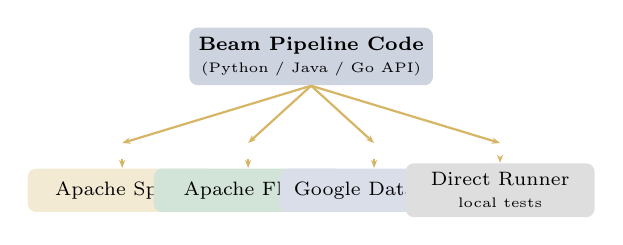
\begin{tikzpicture}[
            box/.style={rectangle, rounded corners=3pt, minimum width=2.4cm,
                        minimum height=0.55cm, font=\scriptsize, align=center},
            arr/.style={-{Stealth[length=3pt]}, draw=PUGold!70, thick}
          ]
          \node[box, fill=PUNavy!20] (code) at (0, 2.5)
                {\textbf{Beam Pipeline Code}\\{\tiny (Python / Java / Go API)}};

          \node[box, fill=PUGold!20]  (ra) at (-2.4, 0.8) {Apache Spark};
          \node[box, fill=PUGreen!20] (rb) at (-0.8, 0.8) {Apache Flink};
          \node[box, fill=PUNavy!15]  (rc) at (0.8,  0.8) {Google Dataflow};
          \node[box, fill=PUGray!20]  (rd) at (2.4,  0.8)
                {Direct Runner\\{\tiny local tests}};

          \foreach \rx/\rn in {-2.4/ra, -0.8/rb, 0.8/rc, 2.4/rd} {
            \draw[arr] (code.south)--(\rx, 1.4);
            \draw[arr, PUGold!70] (\rx, 1.2)--(\rn.north);
          }
        \end{tikzpicture}
        \end{center}
        \vspace{4pt}
        A fraud detection pipeline written in Beam runs in batch mode (Spark) for historical replay and in streaming mode (Flink) in production --- using \textbf{identical business logic code}.  This eliminates the Lambda architecture's synchronisation burden.
      \end{exampleblock}
  \end{columns}
\end{frame}

%================================================================
\section{Ivy League Alignment}
%================================================================

\begin{frame}{Emerging Trends in Top University Curricula}
  \begin{columns}[T]
    \column{0.55\textwidth}
      \begin{block}{MIT 6.830 — Database Systems (Madden, Stonebraker)}
        \small MIT's database course dedicates its final module to \textbf{post-HDFS architectures}:
        \begin{itemize}
          \item The \textbf{Lakehouse vs. data warehouse debate} is a capstone seminar: students read Armbrust (2020) and debate whether Delta Lake renders Snowflake and Redshift obsolete
          \item \textbf{Federated query optimisation} is a graded problem set: students extend a query planner to push predicates across Delta Lake + Postgres + S3 JSON in a single query
          \item The \textbf{Dataflow Model} (Akidau 2015) is required reading, with a lecture devoted to the ``What/Where/When/How'' framework as the theoretical foundation for unified batch/stream
        \end{itemize}
      \end{block}
      \vspace{4pt}
      \begin{exampleblock}{CMU 15-721 — Advanced Database Systems (Pavlo)}
        \small CMU focuses on \textbf{Lakehouse internals}:
        \begin{itemize}
          \item Students implement a subset of the \textbf{Delta Log} (optimistic concurrency using JSON transaction log) as a semester project
          \item \textbf{DuckDB} (in-process analytical engine on Parquet/Delta) is the primary hands-on tool for the Lakehouse module --- replacing Spark for exploratory analysis
        \end{itemize}
      \end{exampleblock}

    \column{0.42\textwidth}
      \begin{alertblock}{Stanford CS329S — ML Systems (Huyen)}
        \small Stanford's ML Systems course is the closest equivalent to our MLOps content:
        \begin{itemize}
          \item \textbf{Hidden Technical Debt} (Sculley 2015) is the first assigned paper; students map every component of the ``debt taxonomy'' onto a real production ML system
          \item \textbf{Feature store design} is a graded project: students implement a time-aware feature store (preventing future data leakage) using Feast on a Kafka--Spark pipeline
          \item The course argues that \textbf{data-centric AI} (improving data quality rather than model architecture) is the highest-leverage activity for production ML engineers --- aligning with Week 2's data integration content
        \end{itemize}
      \end{alertblock}
      \begin{block}{Harvard CS265 — Big Data Systems (Idreos)}
        \small Harvard's final lecture covers \textbf{Data Mesh vs.\ centralised data lake} as an organisational architecture question, assigning Dehghani (2019) and requiring students to recommend an architecture for a fictitious fintech company.
      \end{block}
  \end{columns}
\end{frame}

%================================================================
\section{Student Assessment Pool}
%================================================================

\begin{frame}{Assessment\textemdash MCQ Set A \hfill\small\textit{CLO4}}
  \begin{exampleblock}{Instructions}
    Select the single best answer.  Correct answers \textbf{bolded} for instructor reference.
  \end{exampleblock}
  \vspace{6pt}
  \begin{itemize}
    \item[\textbf{Q1.}] The Lakehouse architecture primarily combines:
    \begin{enumerate}[(a)]
      \item MapReduce batch processing and Apache Hive SQL
      \item \textbf{Data lake flexible storage with data warehouse reliability (ACID transactions and schema enforcement)}
      \item Streaming ingestion and edge analytics
      \item Cloud object storage with in-memory graph processing
    \end{enumerate}
  \end{itemize}
  \vspace{8pt}
  \begin{itemize}
    \item[\textbf{Q2.}] Apache Iceberg and Delta Lake address which fundamental limitation of traditional data lakes?
    \begin{enumerate}[(a)]
      \item Poor compression ratios on object storage
      \item Lack of SQL query support
      \item \textbf{Absence of ACID transactions and schema enforcement, leading to unreliable concurrent writes}
      \item Inability to store unstructured data such as images or documents
    \end{enumerate}
  \end{itemize}
  \vspace{6pt}
  \begin{alertblock}{Instructor Notes}
    \textbf{Q1:} The Lakehouse does not replace streaming (c) or add graph processing (d) --- it unifies lake storage with warehouse reliability.  \textbf{Q2:} Both Delta Lake and Iceberg keep SQL support (b) intact and do not change storage compression (a) --- their core innovation is the transaction log that provides ACID semantics on top of immutable object storage files.
  \end{alertblock}
\end{frame}

%----------------------------------------------------------------
\begin{frame}{Assessment\textemdash MCQ Set B \hfill\small\textit{CLO4}}
  \vspace{6pt}
  \begin{itemize}
    \item[\textbf{Q3.}] The Data Mesh concept was proposed primarily to solve:
    \begin{enumerate}[(a)]
      \item Storage cost problems in HDFS at petabyte scale
      \item Streaming latency issues in Kafka consumer groups
      \item \textbf{Bottlenecks caused by centralised data teams owning and serving all organisational data pipelines}
      \item Security vulnerabilities in Hadoop's authentication model
    \end{enumerate}
  \end{itemize}
  \vspace{8pt}
  \begin{itemize}
    \item[\textbf{Q4.}] Federated Learning is primarily used for:
    \begin{enumerate}[(a)]
      \item Distributed SQL queries across Hive metastore partitions
      \item Real-time event stream processing with sub-second latency
      \item \textbf{Training machine learning models on distributed data without transferring raw data to a central location, preserving privacy}
      \item Graph analytics and community detection on social networks
    \end{enumerate}
  \end{itemize}
  \vspace{6pt}
  \begin{alertblock}{Instructor Notes}
    \textbf{Q3:} Data Mesh is an \textit{organisational} architecture (not a storage or latency solution) that transfers data ownership from a central team to domain teams.  \textbf{Q4:} The defining property of Federated Learning is that \textbf{raw data never moves} --- only model gradient updates are aggregated centrally via FedAvg.  This is the mechanism that makes it privacy-preserving for healthcare and banking.
  \end{alertblock}
\end{frame}

%----------------------------------------------------------------
\begin{frame}{Assessment\textemdash True / False \hfill\small\textit{CLO4}}
  \begin{block}{Instructions}
    State True or False and provide a \textbf{one-sentence justification} for full marks.
  \end{block}
  \vspace{4pt}
  \centering
  \renewcommand{\arraystretch}{1.6}
  \begin{tabular}{p{9.0cm}c}
    \toprule
    \textbf{Statement} & \textbf{Answer} \\
    \midrule
    1.\ Apache Beam allows the same pipeline code to run on both Apache Spark and Apache Flink as backend runners. &
    \textbf{True} \\
    2.\ Cloud-managed services such as AWS EMR require the user to provision and manage Hadoop cluster hardware manually. &
    \alert{\textbf{False}} \\
    3.\ Differential privacy guarantees that individual records cannot be inferred from aggregate query results, at the cost of some accuracy. &
    \textbf{True} \\
    4.\ The Data Mesh approach centralises all data ownership in a single platform team to improve governance and quality. &
    \alert{\textbf{False}} \\
    \bottomrule
  \end{tabular}
  \vspace{6pt}
  \begin{exampleblock}{Model Justifications}
    \small \textbf{2:} AWS EMR is a \textbf{fully managed} service --- AWS provisions, patches, and terminates EC2 instances automatically; the user specifies cluster size and submits Spark/Hive jobs only.  \textbf{4:} Data Mesh is explicitly the \textbf{opposite} --- it \textit{decentralises} data ownership to individual domain teams, removing the central data team as the single point of bottleneck and failure.
  \end{exampleblock}
\end{frame}

%----------------------------------------------------------------
\begin{frame}{Assessment\textemdash Descriptive Questions \hfill\small\textit{CLO4}}
  \begin{block}{Instructions}
    Answer each question in \textbf{100--150 words}.
  \end{block}
  \vspace{6pt}
  \begin{itemize}
    \item[\textbf{D1.}] Explain the \textbf{Lakehouse architecture}.  What specific problems does it solve that neither a pure data lake nor a pure data warehouse could solve individually?  Name one open-source technology that implements the Lakehouse concept and describe its core mechanism.
  \end{itemize}
  \vspace{8pt}
  \begin{itemize}
    \item[\textbf{D2.}] What is \textbf{federated learning}?  Give a specific healthcare example where federated learning is preferable to centralising all patient data on a single cluster.  What are two \textbf{limitations} of federated learning that a system architect must account for?
  \end{itemize}
  \vspace{8pt}
  \begin{itemize}
    \item[\textbf{D3.}] Reflect on the 11-week course: explain how \textbf{HDFS $\to$ MapReduce $\to$ Hive $\to$ Spark $\to$ Kafka $\to$ Lakehouse} forms a coherent and chronologically motivated technology stack.  What was the driving force behind each transition?
  \end{itemize}
\end{frame}

%----------------------------------------------------------------
\begin{frame}{Assessment\textemdash Capstone Analytical Questions \hfill\small\textit{CLO4}}
  \begin{block}{Instructions}
    Answer in \textbf{250--350 words} with full end-to-end pipeline reasoning and explicit tool justification.
  \end{block}
  \vspace{4pt}
  \begin{itemize}
    \item[\textbf{A1.}] \textbf{National Mobile Payment Platform Design:}\\
    Design a complete big data analytics platform for a nationwide mobile payment company in Bangladesh (like bKash) handling 50 million transactions per day.  Your design must include: (a)\ data ingestion layer --- how transactions enter the system; (b)\ storage architecture --- HDFS or Lakehouse on cloud; (c)\ batch analytics layer --- for monthly regulatory reports; (d)\ real-time fraud detection layer --- achieving sub-2-second latency; (e)\ visualisation dashboard.  Name every tool from this course you would use and justify each choice against a specific alternative.
  \end{itemize}
  \vspace{6pt}
  \begin{itemize}
    \item[\textbf{A2.}] \textbf{Ethics --- Social Media Mental Health Prediction:}\\
    A researcher uses 5 years of Facebook posts from 2 million Bangladeshi users (scraped without explicit consent) to train a model predicting depression with 90\% accuracy.  (a)\ What are the privacy and ethical concerns?  (b)\ How could \textbf{federated learning} or \textbf{differential privacy} mitigate these concerns?  (c)\ Should this model be deployed in a hospital setting?  Justify your answer with reference to HIPAA/PDPA principles and the risk of algorithmic bias.
  \end{itemize}
\end{frame}

%================================================================
\section*{Textbook References}
%================================================================

\begin{frame}{Textbook \& Reading References}
  \begin{block}{Primary Textbooks for Week 11}
    \begin{itemize}
      \item \textbf{[SA]}\ Acharya \& Chellappan. \textit{Big Data and Analytics}, Wiley, 2015.
            \hfill\textbf{Ch.\ 1, 12}
            \begin{itemize}
              \small\item Ch.\,12: Future directions in big data; cloud integration; privacy
            \end{itemize}
      \item \textbf{[TE]}\ Erl, Khattak \& Buhler. \textit{Big Data Fundamentals}, Prentice Hall, 2016.
            \hfill\textbf{Ch.\ 14}
            \begin{itemize}
              \small\item Ch.\,14: Big data governance, security, and emerging patterns
            \end{itemize}
      \item \textbf{[MMS]}\ Mayer-Sch\"{o}nberger \& Cukier. \textit{Big Data: A Revolution}, Houghton Mifflin Harcourt, 2013.
            \hfill\textbf{Epilogue}
            \begin{itemize}
              \small\item Risks and responsibilities of big data; datafication and its social consequences
            \end{itemize}
    \end{itemize}
  \end{block}
  \vspace{4pt}
  \begin{exampleblock}{Seminal Papers (covered in Week 11, Part 2)}
    \begin{itemize}
      \small
      \item Armbrust, M.\ et al.\ (2020). \textbf{Delta Lake: High-Performance ACID Table Storage over Cloud Object Stores.} \textit{VLDB 2020.}
      \item Zaharia, M.\ et al.\ (2021). \textbf{Lakehouse: A New Generation of Open Platforms That Unify Data Warehousing and Advanced Analytics.} \textit{CIDR 2021.}
      \item Akidau, T.\ et al.\ (2015). \textbf{The Dataflow Model: A Practical Approach to Balancing Correctness, Latency, and Cost in Massive-Scale, Unbounded, Out-of-Order Data Processing.} \textit{VLDB 2015.}
      \item Sculley, D.\ et al.\ (2015). \textbf{Hidden Technical Debt in Machine Learning Systems.} \textit{NeurIPS 2015.}
    \end{itemize}
  \end{exampleblock}
\end{frame}

%----------------------------------------------------------------
\begin{frame}[c]
  \begin{center}
    {\Large\bfseries Congratulations --- You Have Completed CSE 4345}\\[8pt]
    {\large Week 11, Part 1 $\;\mid\;$ Big Data Analytics}\\[8pt]
    \textcolor{PUGray}{\rule{7cm}{0.5pt}}\\[10pt]
    \begin{quote}
      \itshape ``The world is now awash in data and we can see consumers in a lot clearer ways.''
    \end{quote}
    \hfill\textemdash\ Max Levchin, Co-founder of PayPal

    \vspace{10pt}
    \begin{columns}
      \column{0.48\textwidth}
        \begin{block}{\centering Week 11, Part 2}
          \centering\small
          Seminal Papers: Armbrust 2020 (Delta Lake) $\cdot$ Zaharia 2021 (Lakehouse) $\cdot$ Akidau 2015 (Dataflow Model)\\[4pt]
          \textbf{Case Study:} Databricks Lakehouse in production --- how the company that built Spark now bets the company on Delta Lake
        \end{block}

      \column{0.48\textwidth}
        \begin{alertblock}{\centering Capstone Project Reminder}
          \centering\small
          Final Project + Exhibition is \textbf{10\%} of your grade.\\[4pt]
          Apply one or more tools from this course to a \textbf{Bangladesh-context dataset}.  Present your pipeline, results, and lessons learned.
        \end{alertblock}
    \end{columns}

    \vspace{6pt}
    \textbf{Reading before Part 2:}\ Armbrust et al.\ (2020) --- open access on VLDB website.
  \end{center}
\end{frame}

%=================================================================
\end{document}
%=================================================================
